\documentclass[uplatex]{jsarticle}
\usepackage{nidanfloat}
\usepackage[dvipdfmx]{graphicx}
\usepackage[dvipdfmx]{color}
\usepackage{amsmath}
\newcommand{\argmax}{\mathop{\rm arg~max}\limits}
\newcommand{\argmin}{\mathop{\rm arg~min}\limits}
\title{Topic Sentiment Joint Model with BERT}
\author{東北大学 経済学研究科 C0EM1023 長谷川 一旗}
\date{\today}
\begin{document}
\maketitle

%概要
\begin{abstract}
    \large
    概要を後で書くよ
\end{abstract}
\newpage
\tableofcontents
\twocolumn
\section{Introduction}
高度な情報化社会の成立により、テキストデータが急速に蓄積されつつある現代社会において、テキストから隠れた知見を発見するためのテキストマイニングは非常に多くの分野で活用されている。

マーケティング分野においては、Eコマース事業やソーシャルメディアの急速な発展に伴って、オンライン上に散見されるレビューを分析し、消費者の感情やトピックを抽出し理解することが、企業にとって非常に重要視されつつある。
したがって、テキストから書き手の感情を解析する手法やテキストから書き手の関心ごとであるトピックを抽出するトピックモデルといった手法は、その重要性から近年の主要な研究分野の一つとなっており、様々な改良モデルが考案されている。
Joint Sentiment Topic Model(JST)\cite{JST}では、Latent Dirichlet Allocation(LDA)\cite{LDA}にセンチメント層を導入することで、テキストから感情とトピックを同時に抽出することを可能にし、より実用的なモデルへと拡張している。
Gaussian LDA for Topic Models with Word Embeddings\cite{Gaussian LDA}では、自然言語処理分野において、分散表現(Word Embeddings)と呼ばれる単語を高次元のベクトルで表現する技術をLDAに導入することで、意味的に近く解釈のしやすいトピックの
抽出が可能となったと同時にモデルの性能の向上も示されている。Joint Sentiment Topic Model(JST)では、学習コーパスの少ない場合にモデル性能の低下することが問題として指摘されており、この問題点の解決するために分散表現を導入したTopic Sentiment Joint Model with Word Embeddings\cite{TSWE}というモデルも存在する。
このモデルでは、外部の大規模コーパスを用いた分散表現の導入によって、モデルの性能が大幅に向上したことが示されている。しかしながら、これらのモデルに利用されている分散表現は、Word2Vec\cite{Word2Vec}という文脈を考慮していない分散表現である。文脈を考慮しない分散表現では、異なる意味合いを持つ単語に対して
それぞれの意味を区別できない分散表現になってしまうため、多義語のある文章に対して十分な性能を発揮できないという問題点が指摘されている。近年の自然言語処理分野では、こうした問題点に対応するために深層学習を利用することで文脈を考慮した単語分散表現の獲得を目指す研究が盛んに行われており、ELMo\cite{ELMo}やBERT\cite{BERT}といったモデルは
既存の分散表現モデルと比較して、高い性能を誇ることが知られている。よって、既存の分散表現であるWord2Vecを利用している様々なタスクやモデルにおいて、こうした文脈を考慮した分散表現を置換してあげることにより性能の向上が見込まれるが、それらを検証した論文は多くは出てきていません。

したがって、本稿では分散表現を利用したセンチメントとトピックの同時抽出モデルであるTopic Sentiment Joint Model with Word Embeddings(TSWE)に導入する分散表現として、文脈考慮型の分散表現を導入したモデルを提案し、その有効性について実験を通して検証を行っていく。

%先行研究
\section{Related Researches}
%LDA
\subsection{Latent Dirichlet Allocation(LDA)}
LDAは、Bleiら\cite{LDA}によって提案された文書の確率的生成モデルである。LDAでは、文書には複数のトピックが存在すると仮定し、文書中に含まれる単語にトピックを割り当てる。トピックは、文書から観測できないため、文書内の単語の共起情報からトピックを推定する。
図1(a)に示すLDAの生成過程をまとめると以下の通りである。
\begin{enumerate}
    \item for $k=1$ to $K$
          \begin{enumerate}
              \item Draw word distribution $\phi_{k} \sim $Dir($\beta$)
          \end{enumerate}
    \item For each document $d$
          \begin{enumerate}
              \item Draw a topic distribution $\theta_{d} \sim $Dir($\alpha$)
              \item For each word index n from 1 to $N_{d}$
                    \begin{enumerate}
                        \item Draw a topic $z_{dn} \sim$ Multi($\theta_{d}$)
                        \item Draw a word $w_{dn} \sim$ Multi($\phi_{z_{dn}}$)
                    \end{enumerate}
          \end{enumerate}
\end{enumerate}

LDAは、自然言語処理分野だけでなく多種多様な分野に応用可能なモデルであり、改良も容易であることから様々な改良モデルが存在する。その中でも、センチメント層を導入することで感情推定とトピック推定を同時に行うことを可能にしたモデルであるJST\cite{JST}モデルを2.2節、分散表現を導入することでその性能を向上させただけでなく、未知語に対しても対応可能になっているGaussian LDA\cite{Gaussian LDA}モデルを2.3節で紹介する。
2.4節では、本稿での提案手法の基礎にもなったJSTモデルに分散表現を導入することで、より性能を向上させたTSWE\cite{TSWE}モデルの紹介を行う。
% JST
\subsection{Joint Sentiment/Topic Model for Sentiment Analysis(JST)}
JSTは、Linら\cite{JST}によって提案された文書からセンチメントとトピックの抽出を目的としたモデルである。JSTでは、文書単位での感情分類を達成するために、文書層とトピック層との間にセンチメント層を導入することで通常のLDAモデルを拡張した。
JSTでは、従来のLDAと異なり、$S$個のセンチメントラベルが文書と紐づけられており、そのもとでトピックがセンチメントラベルに紐づけられている。したがって、単語はセンチメントラベルとトピックの両方に紐づけられることになる。
図1(b)に示すJSTの生成過程をまとめると以下の通りである。
\begin{enumerate}
    \item For each topic-sentiment pair ($k$,$l$)
          \begin{enumerate}
              \item Draw word distribution $\phi_{k,l} \sim $ Dir($\beta$)
          \end{enumerate}
    \item For each document $d$
          \begin{enumerate}
              \item Draw a sentiment distribution $\pi_{d} \sim $ Dir($\gamma$)
              \item For $l=1$ to $S$
                    \begin{enumerate}
                        \item Draw a topic distribution $ \theta_{d,l} \sim $ Dir($\alpha$)
                    \end{enumerate}
              \item For each word index n from 1 to $N_{d}$
                    \begin{enumerate}
                        \item Draw a sentiment label $l_{dn} \sim \pi_{d}$
                        \item Draw a topic $z_{dn} \sim \theta_{d, l_{dn}}$
                        \item Draw a word $w_{dn} \sim \phi_{z_{dn},l_{dn}}$
                    \end{enumerate}
          \end{enumerate}
\end{enumerate}

映画のレビューデータセットを利用した評価実験では、他のラベル付きアプローチと比較して、文書レベルでの感情分類において非常に優れた性能を示している。加えて、抽出されたトピックからは確かに一貫したトピックとなっていることも示している。
しかしながら、このモデルでは単語をBag-of-wordsとして表現しているため、単語の順序を考慮出来ていないということが指摘されている。

%Gaussian LDA
\subsection{Gaussian LDA for Topic Models with Word Embeddings}
分散表現学習の登場により、トピックモデルと分散表現を組み合わせ、より意味的に一貫したトピックが生成されやすくなることを目指した研究が、Gaussian LDA\cite{Gaussian LDA}である。
このモデルは、Huら\cite{Gaussian}が提案したLDAにおけるトピックを生成する分布を多次元ガウス分布にするというモデルに単語の分散表現を組み合わせたもので、Dasら\cite{Gaussian LDA}によって提案された。連続空間上に埋め込まれた単語ベクトル
に対して、トピック$k$を同一空間上での多次元ガウス分布とした。これによって、トピック毎の単語分布が連続分布となり、この分布から単語ベクトルが生成される過程がモデル化されている。
図1(c)に示すGaussian LDAの生成過程をまとめると以下の通りである。

\begin{enumerate}
    \item for $k=1$ to $K$
          \begin{enumerate}
              \item Draw topic covariance $\bf{\Sigma_{k}} \sim \mathcal{W}^{-1}(\Psi, \nu)$
              \item Draw topic mean $\bf{\mu_{k}} \sim \mathcal{N}(\bf{\mu}, \frac{1}{\mathcal{K}}\bf{\Sigma_{k}})$
          \end{enumerate}
    \item For each document $d$
          \begin{enumerate}
              \item Draw a topic distribution $\theta_{d} \sim $Dir($\alpha$)
              \item For each word index n from 1 to $N_{d}$
                    \begin{enumerate}
                        \item Draw a topic $z_{dn} \sim$ Categorical($\theta_{d}$)
                        \item Draw $v_{dn} \sim \mathcal{N}(\bf{\mu_{z_{dn}}}, \bf{\Sigma_{z_{dn}}})$
                    \end{enumerate}
          \end{enumerate}
\end{enumerate}

このモデルでは、従来のLDAと異なり単語をBag-og-wordsとして表現するのではなく、分散表現を用いて表現することで、分散表現が類似しているつまり意味的に近しいと思われる単語を同じトピックに割り当てやすくなり、トピック内の意味的統一性が向上し、自己相互情報量(PMI)も上昇することが報告されている。
しかしながら、このモデルで利用されている分散表現はWord2Vec\cite{Word2Vec}と呼ばれる手法を用いて作成されたものである。この手法では、Bag-of-wordsと同じく単語の順序を考慮できていないため、文脈を考慮した結果にならず多義語などの場合に推定がうまくできない可能性が残されている。

\begin{figure*}
    \begin{tabular}{ccc}
        \begin{minipage}[b]{0.33\hsize}
            \begin{center}
                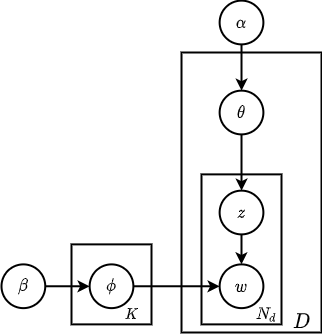
\includegraphics[width=4cm]{picture/LDA.png}
                (a)LDA
            \end{center}
        \end{minipage}
        \begin{minipage}[b]{0.33\hsize}
            \begin{center}
                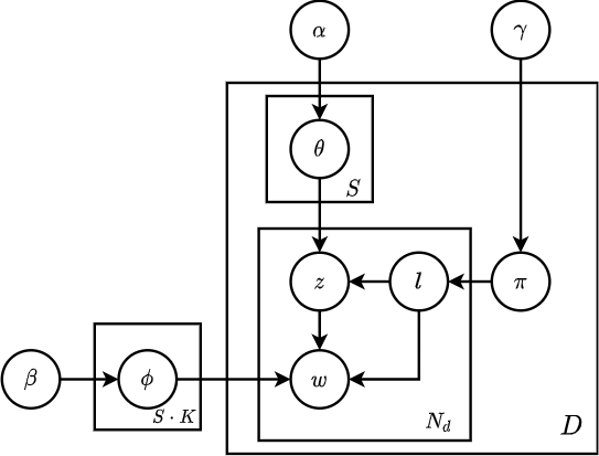
\includegraphics[width=5cm]{picture/JST.png}
                (b)JST
            \end{center}
        \end{minipage}
        \begin{minipage}[b]{0.33\hsize}
            \begin{center}
                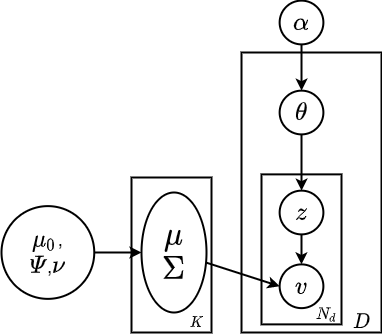
\includegraphics[width=4cm]{picture/GaussianLDA.png}
                (c)Gaussian LDA
            \end{center}
        \end{minipage}
    \end{tabular}
    \caption{グラフィカルモデル}
\end{figure*}

%TSWE
\subsection{Topic and Sentiment Model with Word Embeddings(TSWE)}
TSWEは、JSTに外部の大規模コーパスから学習させた分散表現を導入したJoint Topic Sentiment Modelで、Fuら\cite{TSWE}によって提案されたモデルである。
TSWEでは、学習コーパスが短く小さい場合に、それまでのTopic Sentiment Joint Modelで問題視されていた、単語の共起情報を使用することによって生じる分布の推定がうまくいかない問題を単語の分散表現を導入することにより解決を試みた研究である。
TSWEでは、JSTにおけるディリクレ多項式成分をSentiment-Topic-Wordのディリクレ多項式成分とWord Embeddings成分の混合成分に置換している。
このモデルでは、Word Embeddings成分から単語を生成する確率を以下のように定めている。
\begin{equation}
    MulT(w_{i}|\nu_{k}\omega^{T}) = \frac{{\rm exp}(\nu_{k}*\omega_{w_{i}})}{\Sigma_{w_{i}^{'}\in{W}}{\rm exp}(\nu_{k}*\omega_{w_{i}^{'}})}
\end{equation}

図2に示すTSWEの生成過程をまとめると以下の通りである。

\begin{enumerate}
    \item For each topic-sentiment pair ($l$,$k$)
          \begin{enumerate}
              \item Genearte the word distribution of the sentiment-topic pair $\phi_{l,k} \sim $ Dir($\beta$)
          \end{enumerate}
    \item For each document $d$
          \begin{enumerate}
              \item Draw a distribution $\pi_{d} \sim $ Dir($\gamma$)
              \item For $l=1$ to $S$ under document $d$
                    \begin{enumerate}
                        \item Draw a topic distribution \\ $ \theta_{d,l} \sim $ Dir($\alpha$)
                    \end{enumerate}
              \item For each word index n from 1 to $N_{d}$
                    \begin{enumerate}
                        \item Draw a sentiment label \\ $ l_{dn}  \sim$ Multi($\pi_{d}$)
                        \item Draw a topic $z_{dn} \sim $ Multi($\theta_{d, l_{dn}}$)
                        \item Draw a binary indicator variable \\ $s_{dn} \sim $ Ber($\lambda$)
                        \item Draw a word \\$w_{dn}  \sim (1-s_{dn})$Multi$(\phi_{z_{dn},l_{dn}})+(1 - s_{dn})MulT(\nu_{z_{dn}}\omega^{T}$)
                    \end{enumerate}
          \end{enumerate}
\end{enumerate}

しかしながら、このモデルでもGaussian LDA\cite{Gaussian LDA}同様、分散表現としてWord2Vec\cite{Word2Vec}で学習させた分散表現を用いており、依然として文脈を考慮できないという問題点が残されている。
本研究では、この問題点を解決するために利用する分散表現をBERT\cite{BERT}と呼ばれる手法で学習させた文脈を考慮できる分散表現を用いて、その性能の向上を図る。
こうした点を踏まえ、次節以降では、単語分散表現を獲得する手法として有名なWord2Vec\cite{Word2Vec}や文脈考慮型分散表現の作成をはじめて可能にしたELMo\cite{ELMo}、そのELMoの性能を大幅に向上させただけでなく、汎化性能をも高めたBERT\cite{BERT}について基本的な概念を説明していく。

\begin{figure}[thp]
    \begin{center}
        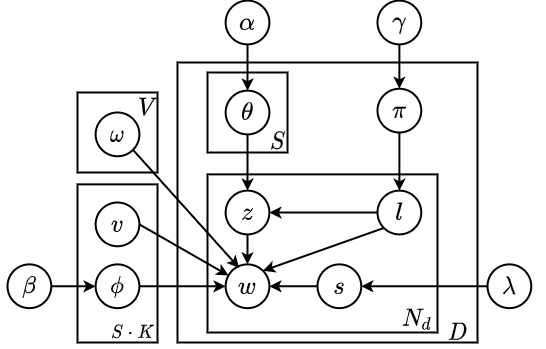
\includegraphics[width=6cm]{picture/TSWE.png}
    \end{center}
    \caption{TSWEのグラフィカルモデル}
\end{figure}
%図の作成or差し替え
\begin{figure}[tbp]
    \begin{center}
        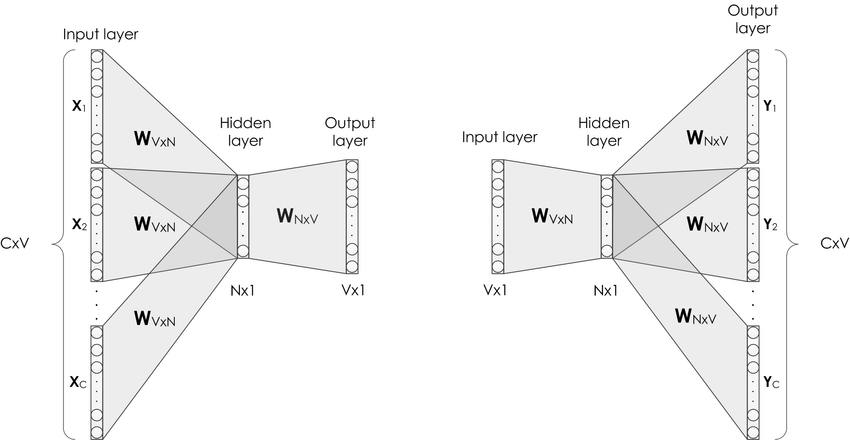
\includegraphics[width=6cm]{picture/Word2Vec.png}
    \end{center}
    \caption{Word2VecにおけるCBOWモデル(左)とSkip-gramモデル(右)\protect\footnotemark[1]}
\end{figure}
\footnotetext[1]{Tutubalinaら\cite{Graph}より引用}


%分散表現の関連研究 Appendixに回すかも
\subsection{Word2Vec}
Word2Vecは、Mikolovら\cite{Word2Vec}が提案したニューラルネットワークを用いて、単語の分布表現を獲得する手法である。つまりは単語を低次元の密なベクトルで表現したものを学習する手法である。
従来、自然言語処理のタスクではテキストデータを扱う際に、bag-of-wordsやLSI\cite{LSI}、pLSI\cite{pLSI}で圧縮したベクトルを用いてきた。しかしながら、これらの手法は次元数が高次元になってしまい計算効率が悪くなってしまう問題点や圧縮した際の精度的な問題点が残されてしまっていた。
こうした問題を解決するため、Mikolovらは単語の意味は単語の周辺の単語によって決定されるという分布仮説の下、テキスト中の各単語を周辺単語から予測するというタスクを設定し、このタスクを大規模なテキストデータからニューラルネットワークによって学習させることで各単語に対する概念ベクトルを獲得した。
Word2Vecには、図3左で示される、周辺の単語から対象とする単語が現れる確率を最大するように学習させる、Countinous Bag-of-Words(CBOW)と呼ばれる手法と図3右で示される、対象の単語を入力とした際の周辺の単語予測のエラー率が最小になるように学習させる、Skip-gramという手法が存在するが、どちらにせよ最終的に単語の分布表現が生成される。
これにより、単語を意味空間上に対応させることができ、意味的に近い単語の分類や単語を意味的に計算することが可能になった。

しかしながら、この手法では対象とする単語とその周辺にどのような単語が存在するかという点しか考慮できず、語順によって異なる意味に捉えられるような単語をうまく表現できないという問題点がある。

コンピュータの計算能力の向上に伴い、深層学習という多層なニューラルネットワークの学習が容易になったことを受け、自然言語処理分野でも凄まじい発展が見られた。
次節で紹介する深層学習を用いた分散表現を獲得する手法を紹介する。

\subsection{ELMo}
ELMoは、Matthewら\cite{ELMo}によって提案された、深層学習を用いることで文脈を考慮した単語の分散表現を獲得する手法である。
ELMoは、LSTM\cite{LSTM}と呼ばれる時系列データを学習することのできるリカレント・ニューラルネットワーク(RNN)の一種を用いた、多層の双方向LSTMによる単語レベルの言語モデルである。
Word2Vecと同様に対象単語の予測確率が高くなるように学習させる点は変わらないが、文頭から対象単語までの順方向と文末から対象単語までの逆方向という双方向の情報を用いて予測させている点がELMoの特徴になっている。
これにより、今まで考慮出来ていなかった文脈を踏まえた分散表現の獲得に成功したのである。加えて、ELMoでは、双方向型言語モデルの中間層によって単語を表現していることも注目すべき点である。

しかしながら、厳密な双方向言語モデルにおいては、予測する単語の先の単語、例えば順方向の場合は対象単語から文末までの単語を事前に知っていることになる。これは、予測においては事前に答えを知っている状態に当たるためうまく予測モデルを作成できないという問題点が生じる。
この問題を解決するために、ELMoでは順方向の情報を用いたモデルと逆方向の情報を用いたモデルを別々に学習させた後、統合する手法が採用されているが、この別々にモデルを学習させている点が浅い双方向モデルと呼ばれ、実際に文脈を捉えているか疑問視されている点でもある。
図4にグラフィカルモデルを示す。

\subsection{BERT}
BERTは、Devlinら\cite{BERT}によって提案された、Transformer\cite{Transformer}という深層学習の手法を用いた様々な自然言語処理タスクに応用可能な事前学習モデルである。
BERTでは、Masked Language Model(MLM)とNext Sentence Prediction(NSP)という二つのタスクを用いて学習させることで、双方向言語モデルにおける学習時に予測対象の先の単語が見えてはいけないという制約を克服した。
MLMは、入力文における15\%の単語に対し、確率的に3つの処理を施した状態でその処理を行う前の単語を予測させるというタスクである。
3つの処理とは、選択された15\%のうち、80\%を[MASK]に置換するマスク変換処理、10\%を別単語に置換する処理、そして残りの10\%は何もせずそのままにする処理となっている。これによって、単語レベルでの学習が可能となっている。
しかしながら、MLMだけでは文レベルでの学習ができないため、次に紹介するNSPというタスクを用いて、文レベルでも学習を行うことで広範な自然言語処理モデルとして機能している。
NSPは、2つの文を入力として与え、その2文が隣り合っているかどうかを当てるタスクである。NSPでは、文の片方を50\%の確率で他の文に置換し、それらが隣り合っているか、隣り合っていないかを判別することで文レベルでの学習を可能としている。

以前から自然言語処理タスクにおける精度の向上には、言語モデルによる事前学習が有効である考えられていた。この言語モデルでは、事前学習で得られた分散表現を特徴量として扱う特徴量ベースという手法と事前学習済みのモデルの最後の部分の重みを再学習させることで新しいタスクにも適用可能にするファインチューニングという手法が存在する。
ELMoは、特徴量ベースであったためタスクに応用する際にそのタスクごとにアーキテクチャを再定義する必要があった。一方、BERTではファインチューニングを採用しているため、タスクごとに大きくパラメータを変更する必要が無く応用の幅が広いという点も特徴の一つである。
図5にグラフィカルモデルを示す。

%図の差し替えor引用の仕方
\begin{figure*}
    \begin{tabular}{cr}
        \begin{minipage}[b]{0.5\hsize}
            \begin{center}
                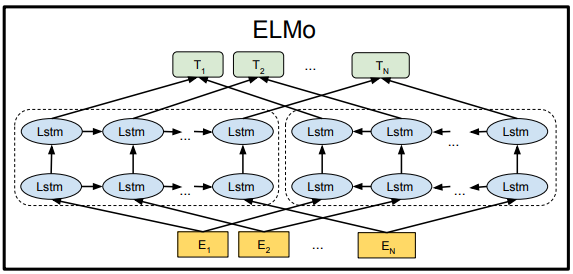
\includegraphics[scale=0.5]{picture/ELMo.png}
                \caption{ELMo}
            \end{center}
        \end{minipage}
        \hspace{1cm}
        \begin{minipage}[b]{0.5\hsize}
            \begin{center}
                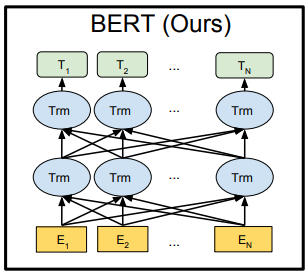
\includegraphics[scale=0.5]{picture/BERT.png}
                \caption{BERT}
            \end{center}
        \end{minipage}
    \end{tabular}
\end{figure*}

%モデルの紹介
\section{Topic and Sentiment Model with BERT}
\subsection{Topic and Sentiment Model with BERT}
本研究では、文脈を考慮できないという問題点の解決のために、文脈も学習させた分散表現を既存のトピックモデルに導入することで、その性能の向上を目指す。
本研究では、マーケティングへの応用という観点からテキストからトピックを抽出することだけでなく、センチメントの抽出も重要だと考え、分散表現を利用したセンチメントとトピックの同時抽出モデルであるTopic Sentiment Joint Model with Word Embeddings(TSWE)\cite{TSWE}を基に、
Word2Vecで学習された分散表現ではなくBERTで学習させた文脈を考慮した分散表現を導入することで、その性能の向上を目指す。また、文脈を考慮した分散表現の導入による性能の向上を測るべく文書レベルでの感情分類タスクとトピック抽出による評価実験を行い、性能について検討していく。

\subsection{Generative process}
\subsection{Gibbs sampling for TSWE model}

%実験&検証
\section{Experiments}
\subsection{Experimental setup}
\subsubsection{Using Word Embeddings}
\subsubsection{Experimental datasets}
\subsection{Parameter Settings}

\subsubsection{Experimental Results and Analysis}


%結論
\section{Conclusions and Future Work}



%\section*{謝辞}
%本研究を進めるにあたり、指導教官である東北大学大学院経済学研究科 石垣 司准教授からは多大な助言を賜りました。この場を借りてお礼申し上げます。
\begin{thebibliography}{数字}
    \bibitem{JST} Lin, C., \& He, Y. (2009). Joint sentiment/topic model for sentiment analysis. International Conference on Information and Knowledge Management, Proceedings, 375–384.
    \bibitem{LDA} Blei, D. M., Ng, A. Y., \& Jordan, M. I. (2003). Latent Dirichlet allocation. Journal of Machine Learning Research, 3(4–5), 993–1022.
    \bibitem{Gaussian LDA} Das, R., Zaheer, M., \& Dyer, C. (2015). Gaussian LDA for topic models with word embeddings. ACL-IJCNLP 2015 - 53rd Annual Meeting of the Association for Computational Linguistics and the 7th International Joint Conference on Natural Language Processing of the Asian Federation of Natural Language Processing, Proceedings of the Conference, 1, 795–804.
    \bibitem{Gaussian} Hu, P., Liu, W., Jiang, W., \& Yang, Z. (2012). Latent topic model based on Gaussian-LDA for audio retrieval. Communications in Computer and Information Science, 321 CCIS, 556–563.
    \bibitem{TSWE} Fu, X., Wu, H., \& Cui, L. (2016). Topic sentiment joint model with word embeddings. CEUR Workshop Proceedings, 1646, 41–48.
    \bibitem{Word2Vec} Mikolov, T., Sutskever, I., Chen, K., Corrado, G., \& Dean, J. (2013). Distributed representations of words and phrases and their compositionality. Advances in Neural Information Processing Systems, 1–9.
    \bibitem{ELMo} Peters, M. E., Neumann, M., Iyyer, M., Gardner, M., Clark, C., Lee, K., \& Zettlemoyer, L. (2018). Deep contextualized word representations. NAACL HLT 2018 - 2018 Conference of the North American Chapter of the Association for Computational Linguistics: Human Language Technologies - Proceedings of the Conference, 1, 2227–2237.
    \bibitem{BERT} Devlin, J., Chang, M. W., Lee, K., \& Toutanova, K. (2019). BERT: Pre-training of deep bidirectional transformers for language understanding. In NAACL HLT 2019 - 2019 Conference of the North American Chapter of the Association for Computational Linguistics: Human Language Technologies - Proceedings of the Conference (Vol. 1).
    \bibitem{LSI} Landauer, T. K., \& Dumais, S. T. (1997). A solution to Plato's problem: The latent semantic analysis theory of acquisition, induction, and representation of knowledge. Psychological Review, 104(2), 211–240.
    \bibitem{pLSI} Hofmann, T. (1999). Probabilistic latent semantic indexing. Proceedings of the 22nd Annual International ACM SIGIR Conference on Research and Development in Information Retrieval, SIGIR 1999, 51(2), 50–57.
    \bibitem{Graph} Tutubalina, Elena \& Nikolenko, Sergey. (2017). Demographic Prediction Based on User Reviews about Medications. Computacion y Sistemas. 21. 227-241. 10.13053/CyS-21-2-2736.
    \bibitem{LSTM} Hochreiter, S. and Schmidhuber, J. (1997). Long Short-Term Memory, Neural Computation, Vol. 9, No. 8, 1735–1780
    \bibitem{Transformer} Vaswani, A., Shazeer, N., Parmar, N., Uszkoreit, J., Jones, L., Gomez, A. N., Kaiser, Ł., \& Polosukhin, I. (2017). Attention is all you need. Advances in Neural Information Processing Systems, 2017-December(Nips), 5999–6009.
\end{thebibliography}
\end{document}
